\section{General Operation}
\label{chp:general_operation}
The \productNumber ~\productName ~features two operation modes. It can be
either operated using the manual user interface or remote controlled by a
computer. In this section the manual operation of the device is explained.

After turning on the \productName ~it comes up with its start screen.
Turning the rotary knob serves to scroll through the menus (see
figure~\ref{main_menu}). Pressing the rotary knob enters the selected
menu. Pressing the menu-escape-button leaves the menu again.

\subsection{Display structure}
In almost every menu four values are displayed. Depending on the previously
selected menu the values correspond to different quantities. Where
\begin{itemize}
  \item the upper left value accompanies to Motor 1
  \item the upper right value accompanies to Motor 2
  \item the lower left value accompanies to Motor 3
  \item the lower right value accompanies to Motor 4
\end{itemize}

\subsection{Motor selection}
To select a motor there are four buttons. Motor selection can solely be done in an entered menu. To select a motor, press the respective motor-selection button. A selected motor is signed with an arrow on the display and by a color change of the corresponding motor-selection button. Pressing the selection-button again deselects the motor. Once a motor is selected its appropriate value can be changed by turning the rotary knob. If multiple motors are selected at the same time, there values will be changed simultaneously. By leaving a menu without motor deselection the selected motor(s) stay selected in any other menu.

\tikzstyle{menu_style} = [rectangle, rounded corners, minimum width=3cm, minimum height=1cm,text centered, draw=black]
\tikzstyle{arrow} = [thick,<->,>=latex]
\def \textWidth {5cm}

\begin{figure}[H]
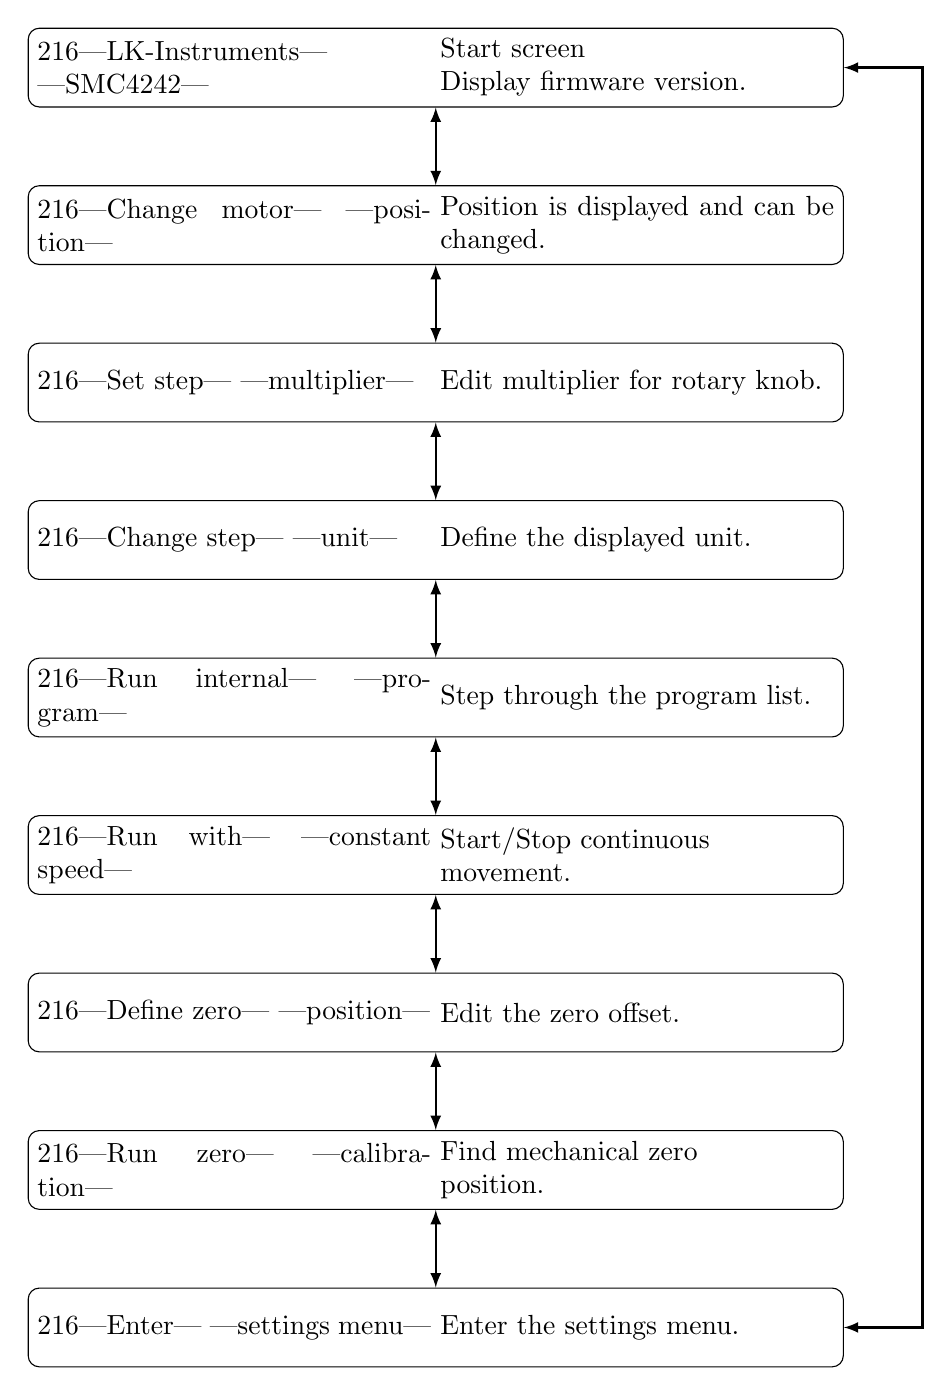
\begin{tikzpicture}[node distance=2cm]
\node (start) [menu_style] {
\begin{minipage}[h]{5cm}
\LCD{2}{16}|LK-Instruments|
|SMC4242|
\end{minipage}
 \hfill
\begin{minipage}[h]{\textWidth}
Start screen\\
Display firmware version.
\end{minipage}
};

\node (motor_pos) [menu_style, below of=start] {
\begin{minipage}[h]{5cm}
\LCD{2}{16}|Change motor|
|position|
\end{minipage}
 \hfill
\begin{minipage}[h]{\textWidth}
%Change motor position:\\
Position is displayed and can be changed.
\end{minipage}
};

\node (step_multiplier) [menu_style, below of=motor_pos] {
\begin{minipage}[h]{5cm}
\LCD{2}{16}|Set step|
|multiplier|
\end{minipage}
 \hfill
\begin{minipage}[h]{\textWidth}
%Set step multiplier\\
Edit multiplier for rotary knob.
\end{minipage}
};

\node (step_unit) [menu_style, below of=step_multiplier] {
\begin{minipage}[h]{5cm}
\LCD{2}{16}|Change step|
|unit|
\end{minipage}
 \hfill
\begin{minipage}[h]{\textWidth}
%Menu: Change step unit\\
Define the displayed unit.
\end{minipage}
};

\node (internal_prog) [menu_style, below of=step_unit] {
\begin{minipage}[h]{5cm}
\LCD{2}{16}|Run internal|
|program|
\end{minipage}
 \hfill
\begin{minipage}[h]{\textWidth}
%Menu: Run internal program\\
Step through the program list.
\end{minipage}
};

\node (const_speed) [menu_style, below of=internal_prog] {
\begin{minipage}[h]{5cm}
\LCD{2}{16}|Run with|
|constant speed|
\end{minipage}
 \hfill
\begin{minipage}[h]{\textWidth}
%Menu: Set constant angular speed\\
Start/Stop continuous\\ movement.
\end{minipage}
};

\node (optical_zero) [menu_style, below of=const_speed] {
\begin{minipage}[h]{5cm}
\LCD{2}{16}|Define zero|
|position|
\end{minipage}
 \hfill
\begin{minipage}[h]{\textWidth}
%Menu: Define optical zero position\\
Edit the zero offset.
\end{minipage}
};

\node (zero_cal) [menu_style, below of=optical_zero] {
\begin{minipage}[h]{5cm}
\LCD{2}{16}|Run zero|
|calibration|
\end{minipage}
 \hfill
\begin{minipage}[h]{\textWidth}
%Menu: Run zero calibration\\
Find mechanical zero\\ position.
\end{minipage}
};

\node (settings) [menu_style, below of=zero_cal] {
\begin{minipage}[h]{5cm}
\LCD{2}{16}|Enter|
|settings menu|
\end{minipage}
 \hfill
\begin{minipage}[h]{\textWidth}
Enter the settings menu.
\end{minipage}
};



\draw [arrow] (start) -- (motor_pos);
\draw [arrow] (motor_pos) -- (step_multiplier);
\draw [arrow] (step_multiplier) -- (step_unit);
\draw [arrow] (step_unit) -- (internal_prog);
\draw [arrow] (internal_prog) -- (const_speed);
\draw [arrow] (const_speed) -- (optical_zero);
\draw [arrow] (optical_zero) -- (zero_cal);
\draw [arrow] (zero_cal) -- (settings);
\draw [arrow] (settings.east) -- +(1,0) |- (start.east);
\end{tikzpicture}
\caption[Overview of the available menus.]{Overview of the available menus. By turning
the rotary knob one can navigate through the menus as indicated by the arrows.}
\label{main_menu}
\end{figure}

\FloatBarrier



\subsection{Start screen}
By pressing the rotary knob while the start screen is active the
firmware version will be displayed.
\begin{center}
  \LCD{2}{16}|SMCx242|
             |Firmware 1.5|
\end{center}
Firmware updates are available at \url{http://www.lk-instruments.com} on
the corresponding product website.

%\begin{macrocode}
%\DefineLCDchar{degree}{11100101001110000000000000000000000}
%\end{macrocode}

\subsection{Motor position}
\label{menu_motor_pos}
\index{change!position}
This menu displays the current motor positions and allows them to be changed. The default display unit is degree, which can be changed to the users preferred unit, see \ref{chp:change_step_unit}. The position of a selected motor can be changed by turning the rotary knob.\\
Default steps for the available units are:
\begin{itemize}
\item $1\degree$ if unit is degree
\item $\frac{\pi}{8}$ if unit is radian
\item 1 step if unit is steps
\end{itemize}
\begin{center}
  \LCD{2}{16}|{rarrow}0.0{pi}   {rarrow}0.0{degree} |
             |{rarrow}0st    {rarrow}0.0{degree} |
\end{center}


\paragraph{Fast moving mode}
\index{fast moving mode}
When pressing the rotary knob inside the change-motor-position-menu one enters the fast moving mode. Pressing the rotary knob again disables the fast moving mode. The fast moving mode is indicated by another marking arrow for the corresponding motor.\\
%The fast moving mode will only be enabled or disabled for selected motors.
Default steps in this mode are:
\begin{itemize}
  \item $10\degree$ if unit is degree
  \item $\frac{\pi}{8}$ if unit is radian
  \item 100 steps if unit is steps
\end{itemize}
The snapped display shows the different indicating arrows.
\begin{center}
  \LCD{2}{16}|>10.0{degree} >0.0{degree} |
             |>0.0{degree}  >0.0{degree} |
\end{center}


\subsection{Step multiplier}
\index{step multiplier}
In this menu the step multipliers can be adjusted. If the step multiplier differs from 1.0 the corresponding motor will rotate more or less steps with each click of the rotary knob. It is also possible to turn the motors in different directions by applying a negative step multiplier to a motor. A step multiplier can only be applied if the step unit is degree or radians. The factory default value for all motors is 1.0.\\
Example: If the step multiplier for motor 1 is 1.0, the step multiplier for motor 2 is 4.0 and the step multiplier for motor 3 is -2.0, when changing the motors positions motor 2 will move four times more steps than motor 1 and motor 3 will move twice as many steps as motor 1, but in the opposite direction. 
%Negative values are allowed as well. This will result in counter direction movements.
\begin{center}
  \LCD{2}{16}|{rarrow}1.0x   {rarrow}4.0x|
             |{rarrow}-2.0x   1.0x|
\end{center}

\subsection{Step unit}
\label{chp:change_step_unit}
\index{change!unit}
In this menu one can choose the unit of the displayed position. Note, that changing the unit will also affect the step width, see~\ref{menu_motor_pos}. There are three possible choices for each motor:
\begin{itemize}
\item degree
\item radian
\item step
\end{itemize}
\begin{center}
  \LCD{2}{16}|{rarrow}radian {rarrow}degree|
             |{rarrow}step    degree|
\end{center}

\subsection{Internal program}
\index{internal program}
This menu allows the user to step through the internal program list with the rotary knob.
This function is only available if a program has previously been defined (see \ref{section_instruction_set}).
Internal programs are also saved to the device when the current configuration is saved, see \ref{menu_save}.
\begin{center}
  \LCD{2}{16}|Program running|
             |Step 0|
\end{center}

\subsection{Constant movement}
Here the motors can be set into an infinite moving state in clockwise (CW) or counter clockwise (CCW) direction. To get the motors moving with different velocities one needs to change the wait times between two steps (see \ref{menu_step_wait_time}).
STOP means that the motor is not moving. Constant speed for a certain motor can not be activated if a forbidden zone is configured for this motor (see \ref{chp:forbidden_zone}).
\begin{center}
  \LCD{2}{16}|{rarrow}CW     {rarrow}CCW|
             | STOP    STOP|
\end{center}

\subsection{Zero position}
\index{zero!position}
In this menu one can define an offset for the zero position. This is necessary due to a mostly unknown placement of the load mounted to a stage. 
%Here one can once adjust the desired optical zero position manually. 
The zero position is always defined in steps. In this menu there is also a fast mode available (please refer to  \ref{menu_motor_pos} for details about the fast mode). After adjustment it is recommended to save this configuration (see \ref{menu_save}). When performing a zero calibration, as explained in \ref{menu_zero_cal}, the zero position will have the defined offset form the mechanical zero position.
\begin{center}
  \LCD{2}{16}|{rarrow}122st   0st|
             | 0st     0st|
\end{center}

\subsection{Zero calibration}
\label{menu_zero_cal}
\index{zero!calibration}
Here one can calibrate the motor zero position for each motor. To perform a zero calibration select the motors to be calibrated and turn the rotary knob. Note, that during zero calibration no actions can be done on the device, even serial commands will not be accepted. The zero calibration will automatically deselect a motor when its calibration is finished. The zero calibration menu will be automatically leaved when calibration is finished.
\begin{center}
  \LCD{2}{16}|{rarrow}Mot 1  {rarrow}Mot 2|
             | Mot 3   Mot 4|
\end{center}

\subsection{Settings menu}
\label{menu_settings}
\index{settings}
The settings menu contains several submenus that allow the user to adjust some of the settings.\\
Turning the rotary knob serves to scroll through the settings menus (see figure~\ref{settings_menu}). Pressing the rotary knob enters the selected settings menu. Pressing the menu-escape-button leaves the settings menu.

\begin{figure}[H]
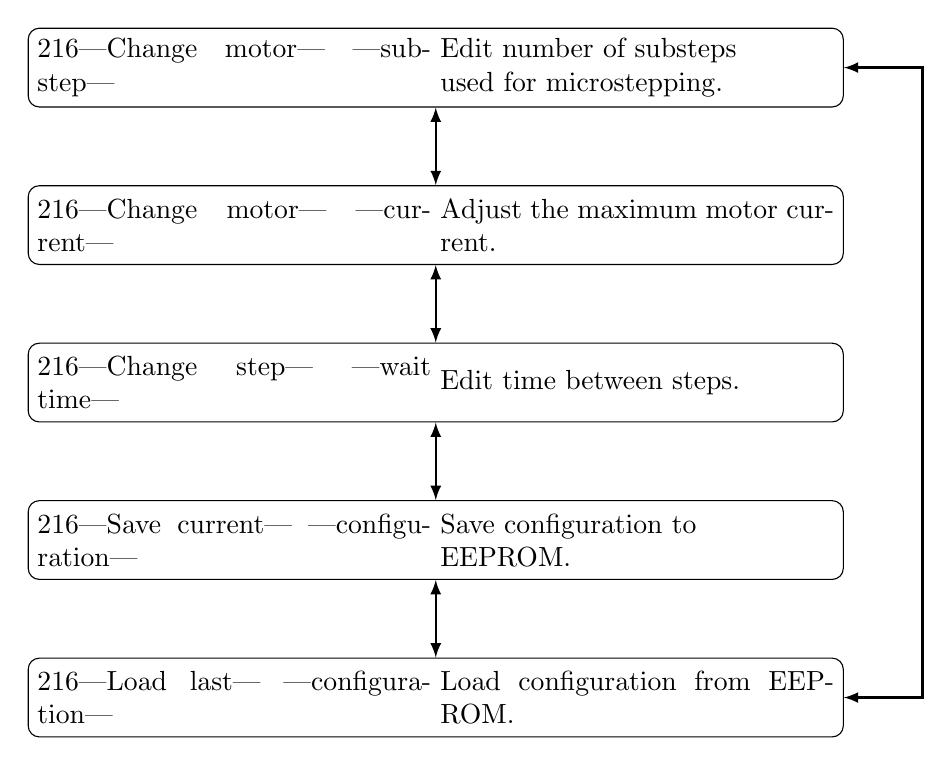
\begin{tikzpicture}[node distance=2cm]
\node (substep) [menu_style] {
\begin{minipage}[h]{5cm}
\LCD{2}{16}|Change motor|
|substep|
\end{minipage}
 \hfill
\begin{minipage}[h]{\textWidth}
%Menu: Change motor substep\\
Edit number of substeps\\ used for microstepping.
\end{minipage}
};

\node (motor_curr) [menu_style, below of=substep] {
\begin{minipage}[h]{5cm}
\LCD{2}{16}|Change motor|
|current|
\end{minipage}
 \hfill
\begin{minipage}[h]{\textWidth}
Adjust the maximum motor current.
\end{minipage}
};

\node (step_wait_time) [menu_style, below of=motor_curr] {
\begin{minipage}[h]{5cm}
\LCD{2}{16}|Change step|
|wait time|
\end{minipage}
 \hfill
\begin{minipage}[h]{\textWidth}
%Menu: Change step wait time\\
Edit time between steps.
\end{minipage}
};

\node (save) [menu_style, below of=step_wait_time] {
\begin{minipage}[h]{5cm}
\LCD{2}{16}|Save current|
|configuration|
\end{minipage}
 \hfill
\begin{minipage}[h]{\textWidth}
%Menu: Save all current configurations\\
Save configuration to\\ EEPROM.
\end{minipage}
};

\node (load) [menu_style, below of=save] {
\begin{minipage}[h]{5cm}
\LCD{2}{16}|Load last|
|configuration|
\end{minipage}
 \hfill
\begin{minipage}[h]{\textWidth}
%Menu: Load last configuration\\
Load configuration from EEPROM.
\end{minipage}
};

\draw [arrow] (substep) -- (motor_curr);
\draw [arrow] (motor_curr) -- (step_wait_time);
\draw [arrow] (step_wait_time) -- (save);
\draw [arrow] (save) -- (load);
\draw [arrow] (load.east) -- +(1,0) |- (substep.east);
\end{tikzpicture}
\caption[Overview of the settings menus.]{Overview of the settings menus. By turning
the rotary knob one can navigate through the settings menus as indicated by the arrows.}
\label{settings_menu}
\end{figure}



\subsubsection{Motor substeps}
\label{menu_substeps}
\index{change!substeps}
\index{change!microstepping}
In this menu one can change the number of substeps used for microstepping. Possible values are 1, 2, 4, 8, 16 or 32.\\
Note, that a value of 1 is equivalent to full step operation. So no microstepping is used to drive the stepper motor. If the adjusted value differs from 1, microstepping is used to obtain finer positioning resolution. Values above 8 are not recommended because of the decreasing motor torque.
\begin{center}
  \LCD{2}{16}|{rarrow}1      {rarrow}2|
             | 4      {rarrow}8|
\end{center}

\paragraph{A note on microstepping.}
\index{microstepping}
When increasing the number of substeps (microsteps per full step) the incremental torque per microstep decreases heavily. The expression for calculating the incremental tourque $\tau_{\text{inc}}$ is
\begin{equation*}
  \tau_{\text{inc}} = \tau_{\text{H}} \cdot \sin \left( \frac{90}{\mu} \right),
\end{equation*}
where $\tau_{\text{H}}$ is the holding torque per full step (without microstepping) and $\mu$ is the number of microsteps per full step.\\
The incremental torque $\tau_{\text{N}}$ for $N$ microsteps is
\begin{equation*}
  \tau_{\text{N}} = \tau_{\text{H}} \cdot \sin \left( \frac{90\cdot N}{\mu} \right).
\end{equation*}
So, the holding torque per microstep decreases as shown in table \ref{tab:microstepping_holding_torque}.
\begin{table}
  \centering
  \begin{tabular}{cc}
    \toprule
    \textbf{Microsteps per full step} & \textbf{Holding torque per microstep} \\
    \toprule
    1 & 100 \% \\ \midrule
    2 & 70.7 \%\\ \midrule
    4 & 38.3 \% \\ \midrule
    8 & 19.5 \% \\ \midrule
    16 & 9.8 \% \\ \midrule
    32 & 4.9 \% \\
    \bottomrule
  \end{tabular}
  \caption{Decrease of motor holding torque in dependence of the number of adjusted microsteps.}
  \label{tab:microstepping_holding_torque}
\end{table}

\subsubsection{Motor current}
\label{menu_motor_current}
\index{change!current}
In this menu the user can change the maximum current that is used to drive the corresponding stepper motor. Please ensure, that the value set here does not exceed the maximum ratings of your motor. 
\begin{center}
  \LCD{2}{16}| 1.0 A  {rarrow}1.3 A|
             |{rarrow}0.9 A   0.5 A|
\end{center}

\subsubsection{Step wait time}
\label{menu_step_wait_time}
\index{change!step wait time}
Here the wait time between two steps can be changed. This results in faster or slower movements of the stepper motor. The default value is 3 milliseconds.\\
Note, that a very short wait time and therefore fast movement speed can lead to stalling of the stepper motor.
%We do not recommend to use shorter wait times as 3 milliseconds.
\begin{center}
  \LCD{2}{16}|{rarrow}3 ms   {rarrow}5 ms|
             |{rarrow}18 ms   3 ms|
\end{center}

\subsubsection{Save current configuration}
\label{menu_save}
\index{save}
To save the current \productName ~configuration enter this menu and turn the rotary knob in any direction.\\
%The menu will be automatically leaved when saving is finished.
Note, that always the configuration for all motors will be saved. It is not possible to save the configuration for a single motor only.
\begin{center}
  \LCD{2}{16}|Save all current|
             |configurations|
\end{center}


\subsubsection{Load configuration}
\label{chp:menu_load}
\index{load}
To load the last saved \productName ~configuration enter this menu and turn the rotary knob in any direction.\\
%The menu will be leaved automatically when loading has finished.
Note: The last saved configuration is loaded automatically when powering on or resetting the \productName.\\
Note: There is just one memory space for a configuration.
\begin{center}
  \LCD{2}{16}|Load all saved|
             |configurations|
\end{center}


%\subsection{Forbidden zones}
%\label{chp:forbidden_zone}

%\subsection{Positioning procedures}
%\label{chp:positioning_procedure}





%\newpage
